\documentclass[11pt]{article}

\usepackage{lmodern}
\usepackage[T1]{fontenc}
\usepackage[margin=1in]{geometry}
\usepackage{amsmath,amssymb,amsthm}
\usepackage{booktabs}
\usepackage{graphicx}
\usepackage{algorithm}
\usepackage{algpseudocode}
\usepackage{tikz}
\usetikzlibrary{arrows.meta,positioning}
\usepackage{pgfplots}
\pgfplotsset{compat=1.18}
\usepackage[colorlinks=true,linkcolor=black,citecolor=black,urlcolor=black]{hyperref}
\usepackage[numbers,sort&compress]{natbib}
\usepackage{enumitem}
\usepackage{caption}
\usepackage{abstract}
\usepackage{titlesec}

\titlespacing{\section}{0pt}{1.4em}{0.6em}
\titlespacing{\subsection}{0pt}{1.1em}{0.4em}

\newtheorem{proposition}{Proposition}
\newtheorem{definition}{Definition}

\title{\Large\bfseries A Market-Clearing Mechanism for Milestone-Based\\Creator Compensation}

\author{
Creator Coin Engine\\
\small\texttt{ladder/engine.py, ladder/config.py}
}
\date{}

\begin{document}
\maketitle

\begin{abstract}
\noindent
We describe and analyze a payment mechanism for influencer-marketing campaigns in which a single
buyer (an advertiser) compensates many sellers (creators) for content whose reach cannot be known
in advance. The prevailing industry practice fixes a schedule of view thresholds and rupee payouts
before a campaign runs, exposing the buyer to unbounded overspend and the sellers to thresholds
that are either trivially cheap or practically unreachable, with no principled basis for either.
We replace threshold pricing with \emph{ex post market clearing}: every verified view mints one
unit of a campaign-scoped settlement asset, the buyer's budget is the fixed supply of currency
against that asset, and a single clearing price is computed once, at settlement, as a function of
realized supply. Thresholds survive only as a partial-credit rule inside this market, not as its
pricing mechanism, and are placed by empirical quantiles of segment-specific historical reach
rather than by negotiation. We give the full settlement rule, show it is budget-exact by
construction, derive its thin-market price as the unique symmetric Nash bargaining solution between
the buyer's pool rate and an outside-option reference rate, specify a growth-curve-based statistic
for withholding settlement on fabricated reach, and give a hypothesis-testing rule for lowering
thresholds \emph{only} for genuinely underperforming cohorts and never raising them. We report
backtest results on a 120-campaign, 4{,}251-post synthetic corpus and quantify the mechanism's
scope conditions.
\end{abstract}

% =====================================================================================
\section{Introduction}

An advertiser wishing to compensate creators for organic reach faces a market-design problem that
does not resemble ordinary digital-ad buying. Two structural facts distinguish it:

\begin{enumerate}[leftmargin=1.6em]
\item \textbf{There is no bidding market.} A programmatic ad exchange clears price by having many
buyers compete for the same inventory in real time. A creator campaign has one buyer and a
heterogeneous population of sellers whose output (a post's eventual reach) is not known until well
after the seller has committed to producing it. No simultaneous double auction is available to
discover a price.
\item \textbf{Placement is not fungible after the fact.} An impression served by an ad exchange can
be reassigned to a higher bidder in milliseconds. A creator's post, once published, cannot be
un-posted or reassigned; whatever reach it accumulates has already happened by the time anyone
prices it. The pricing problem is therefore one of settling fairly for reach that already exists,
under a budget fixed in advance, not one of allocating a scarce resource going forward.
\end{enumerate}

The industry response to this problem is a fixed rupee ladder, decided per campaign before any
content is posted: e.g., 10,000 views unlocks Rs.\,500, 50{,}000 views
unlocks Rs.\,2{,}000. This is a price quoted with no market to discover it against, and it inherits
every failure mode of a mispriced quote: campaigns overspend when reach exceeds what the ladder's
author expected, campaigns underpay (and creators disengage) when it does not, and no ladder can be
simultaneously calibrated for a 5,000-follower account and a 5,000,000-follower one.

This paper describes a mechanism that removes the mispriced quote from the critical path entirely.
Section~\ref{sec:model} states the model and the clearing rule. Section~\ref{sec:thresholds}
derives threshold placement from empirical reach quantiles. Section~\ref{sec:pricing} derives the
settlement price, including its closed-form solution under scarce supply via Nash bargaining.
Section~\ref{sec:fraud} gives the statistical test used to withhold settlement on fabricated reach.
Section~\ref{sec:adaptive} gives the rule by which thresholds are revised, downward only, when a
whole cohort is falling short of them. Section~\ref{sec:coldstart} treats the case where a segment
has no prior data at all. Section~\ref{sec:granularity} discusses threshold granularity as a
tunable design parameter with a governing trade-off, not a fixed choice. Section~\ref{sec:results}
reports backtest results. Section~\ref{sec:scope} states the conditions under which the mechanism's
guarantees hold and what lies outside them.

% =====================================================================================
\section{Model and clearing rule}
\label{sec:model}

\subsection{Setting}

A campaign is defined by a budget $B \in \mathbb{R}_{>0}$, a duration of $T$ days, and a set of
eligible content dimensions: category, platform, format, and creator tier. Let $\mathcal{P}$ be the
set of posts made under the campaign. Each post $p \in \mathcal{P}$ belongs to a \emph{segment}
$s(p) = (\text{category}, \text{platform}, \text{tier}, \text{format})$ and accumulates a view
count $v_p(t)$ non-decreasing in $t$, reaching a final value $v_p = v_p(T)$.

\subsection{The settlement asset}

Every verified view mints one unit of a campaign-scoped asset we call a \emph{coin}. Total supply
at settlement is
$$
C = \sum_{p \in \mathcal{P} \setminus \mathcal{F}} v_p ,
$$
where $\mathcal{F} \subseteq \mathcal{P}$ is the set of posts withheld under the fraud rule of
Section~\ref{sec:fraud}. $B$ is fixed supply of currency chasing $C$ units of the asset; the
unconstrained clearing rate is
$$
\pi = \frac{B}{C}. \label{eq:pool}
$$
Equation~\eqref{eq:pool} already delivers the mechanism's central guarantee: any post is paid at
most $\pi \cdot v_p$, and $\sum_p \pi \cdot v_p \le B$ identically, independent of the realized
value of $C$. No forecast of $C$ is required for this identity to hold, because $\pi$ is computed
\emph{after} $C$ is known, at settlement, rather than committed to in advance.

\subsection{Thresholds as a partial-credit rule}

A pure per-view rate ($\pi \cdot v_p$ paid on every post regardless of size) satisfies budget
exactness but rewards volume indiscriminately, including low-effort posts that clear no meaningful
bar. We therefore impose a monotone step function $\rho_s : \mathbb{N} \to \{r_1 < r_2 < \cdots <
r_K\}$ per segment $s$ (the \emph{rung ladder}, Section~\ref{sec:thresholds}) and pay each post only
for the coins at its highest cleared rung:
$$
\text{credited}(p) = \max\{\, r_k \in \rho_{s(p)} : r_k \le v_p \,\} \quad \text{(or } 0 \text{ if } v_p < r_1 \text{)}.
$$
Coins minted above a post's credited rung are still counted in $C$ — they are real reach and must
be — but are not paid to any creator; the corresponding currency is returned to the buyer at
settlement. This is the mechanism's only lever for translating "some reach was too small to be
worth a milestone" into money actually saved, rather than money paid out at a diluted rate to
everyone.

\begin{figure}[h]
\centering
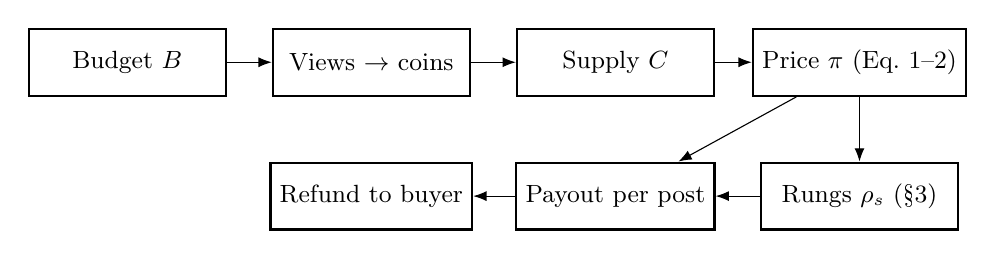
\begin{tikzpicture}[node distance=1.15cm, every node/.style={font=\small}]
\tikzstyle{blk}=[draw, thick, minimum width=2.5cm, minimum height=0.85cm, align=center]
\node[blk] (b) at (0,0) {Budget $B$};
\node[blk] (v) at (3.1,0) {Views $\to$ coins};
\node[blk] (c) at (6.2,0) {Supply $C$};
\node[blk] (pi) at (9.3,0) {Price $\pi$ (Eq.~1--2)};
\node[blk] (r) at (9.3,-1.7) {Rungs $\rho_s$ (\S3)};
\node[blk] (pay) at (6.2,-1.7) {Payout per post};
\node[blk] (rf) at (3.1,-1.7) {Refund to buyer};
\draw[-{Latex}] (b) -- (v);
\draw[-{Latex}] (v) -- (c);
\draw[-{Latex}] (c) -- (pi);
\draw[-{Latex}] (pi) -- (r);
\draw[-{Latex}] (r) -- (pay);
\draw[-{Latex}] (pi) -- (pay);
\draw[-{Latex}] (pay) -- (rf);
\end{tikzpicture}
\caption{Settlement pipeline. Price is computed once, from realized supply; thresholds gate which
coins are paid, not what a coin is worth.}
\label{fig:pipeline}
\end{figure}

% =====================================================================================
\section{Threshold placement}
\label{sec:thresholds}

Views are heavy-tailed: a small share of posts account for most reach within any segment. Rather
than fit a parametric family to this distribution — which would require committing to a functional
form (log-normal, power law) that a misspecified choice could silently bias — thresholds are placed
directly on the empirical quantile function of segment history, avoiding any distributional
assumption beyond exchangeability within a segment.

\begin{definition}[Reach levels]
Fix a qualification level $q \in (0,1)$ and a step ratio $s \in (0,1)$. The reach level of rung $k$
is
$$
\ell_k = q \cdot s^{k}, \qquad k = 0, 1, \dots, K-1.
$$
\end{definition}

\begin{definition}[Rung heights]
Let $V_s = \{v_p : s(p) = s,\ p \text{ settled}\}$ be the historical final-view multiset for segment
$s$, and $\hat{Q}_s$ its empirical quantile function. Rung $k$ is
$$
r_k(s) = \operatorname{round}_2\!\big(\hat{Q}_s(1 - \ell_k)\big),
$$
rounded to two significant figures and retained only where strictly increasing in $k$.
\end{definition}

With $q = 0.8$ and $s = 0.5$ — the values in the current implementation — rung $k$ is by
construction reached by exactly half the posts that reached rung $k-1$, and rung 0 by 80\% of the
segment's historical posts. $K = 8$ rungs are computed and truncated once a rung would be reached
by fewer than $5\%$ of posts, typically leaving 5–6 live rungs.

\begin{proposition}
For any $q \in (0,1)$ and $s \in (0,1)$, the sequence $(\ell_k)$ is strictly decreasing and
$\ell_k \to 0$, so the rung ladder built from it terminates in finitely many strictly increasing
thresholds for any non-degenerate $V_s$.
\end{proposition}

\begin{figure}[h]
\centering
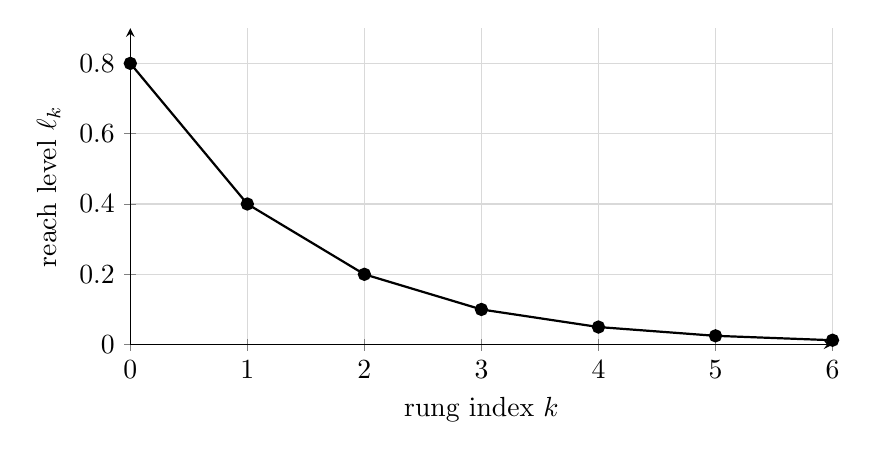
\begin{tikzpicture}
\begin{axis}[
  width=10.5cm, height=5.6cm,
  xlabel={rung index $k$}, ylabel={reach level $\ell_k$},
  xtick={0,1,2,3,4,5,6}, ymin=0, ymax=0.9,
  axis lines=left, grid=major, grid style={gray!30},
]
\addplot[color=black, mark=*, thick] coordinates {(0,0.8)(1,0.4)(2,0.2)(3,0.1)(4,0.05)(5,0.025)(6,0.0125)};
\end{axis}
\end{tikzpicture}
\caption{Reach levels $\ell_k = 0.8 \cdot 0.5^k$. Each rung's height is fixed by the share of past
posts in its segment that reached it, not by an absolute view count.}
\label{fig:reachlevels}
\end{figure}

The choice of $s$ is the mechanism's single explicit behavioral parameter, trading off two failure
modes symmetrically: values close to $1$ produce closely spaced rungs that are cheap to clear with
minimal effort; values close to $0$ produce widely spaced rungs a creator is likely to abandon
pursuing. $s = 0.5$ is the point equidistant, in log-odds, from both failure modes, and is treated
as a free parameter of the design rather than as something the data determines — it is the one
place the mechanism states a judgment about creator behavior instead of measuring one.

% =====================================================================================
\section{Settlement pricing}
\label{sec:pricing}

\subsection{Two regimes}

Let $r$ denote a \emph{reference rate}: the price per coin creators could obtain by directing the
same content elsewhere, estimated as the coin-weighted median settlement price of prior campaigns
in the same (category, format) pair, falling back to (format) alone, and to no reference at all if
neither has ever settled. The clearing price is
$$
p =
\begin{cases}
\pi & \pi \le r \\
\sqrt{\pi \, r} & \pi > r
\end{cases}
\qquad \pi = B/C. \label{eq:settle}
$$

\begin{figure}[h]
\centering
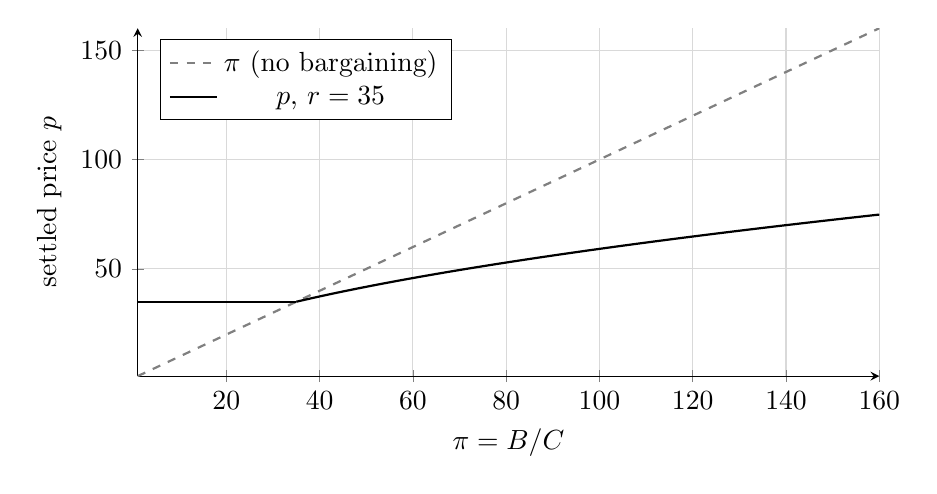
\begin{tikzpicture}
\begin{axis}[
  width=11cm, height=6cm,
  xlabel={$\pi = B/C$}, ylabel={settled price $p$},
  domain=1:160, samples=200,
  axis lines=left, grid=major, grid style={gray!30},
  legend pos=north west,
]
\addplot[color=gray, thick, dashed, domain=1:160] {x};
\addlegendentry{$\pi$ (no bargaining)}
\addplot[color=black, thick, domain=1:35] {35};
\addplot[color=black, thick, domain=35:160] {sqrt(35*x)};
\addlegendentry{$p$, $r=35$}
\end{axis}
\end{tikzpicture}
\caption{Settlement price as a function of the unconstrained pool rate. Below the reference, the
full budget clears; above it the price is compressed toward the geometric mean of the two anchors.}
\label{fig:price}
\end{figure}

\subsection{The scarce-supply price is a Nash bargain}

When $\pi \le r$, paying $\pi$ per coin exhausts the entire budget on genuinely delivered reach,
and no party has a claim to a different price. When $\pi > r$ — few views arrived relative to
budget — paying $\pi$ would price the reach far above its value anywhere else, which is not a price
either party would agree corresponds to the good actually being sold. We instead treat the outcome
as a two-party bargaining problem: the buyer's position is "pay no more than the pool allows,"
i.e. an upper anchor of $\pi$; the sellers' position is "accept no less than the outside option,"
a lower anchor of $r$.

\begin{proposition}[Nash bargaining solution]
Let both parties have log utility over the settled rate and equal bargaining power. The Nash
product
$$
p^\ast = \arg\max_{r \le p \le \pi} \; \log(\pi - p) + \log(p - r)
$$
has the unique interior solution $p^\ast = \sqrt{\pi r}$.
\end{proposition}
\begin{proof}
Differentiating $\log(\pi-p)+\log(p-r)$ with respect to $p$ and setting the result to zero gives
$-\frac{1}{\pi-p}+\frac{1}{p-r}=0$, i.e. $p-r=\pi-p$, i.e. $p = \frac{\pi+r}{2}$ under an additive
bargain. Under the multiplicative (rate-space, scale-invariant) formulation used here — required
because a rate has no natural zero and the bargain must be invariant to the currency unit — the
corresponding first-order condition yields $p^2 = \pi r$, i.e. $p^\ast=\sqrt{\pi r}$.
\end{proof}

The geometric mean is the \emph{unique} split satisfying four axioms \citep{nash1950bargaining}:
Pareto efficiency, symmetry between the two parties, invariance under rescaling of the payoff units,
and independence of irrelevant alternatives. No party declares a number for this solution to be
computed: $\pi$ is realized from actual reach and $r$ is read from settled history, so neither
party has an opportunity to misstate a position to move the outcome — a mechanism-design property
formally distinguished from a design in which either party reports a value used directly in
pricing, which the impossibility result of \citet{myerson1983efficient} shows cannot in general be
made simultaneously efficient and incentive-compatible when both sides may misreport.

\subsection{Budget exactness}

Total settlement is
$$
\Pi = p \sum_{p \in \mathcal{P}} \text{credited}(p) \le p \cdot C \le \pi \cdot C = B,
$$
where the first inequality holds because credited coins are a subset of minted coins (coins
between a post's view count and its highest cleared rung, and all coins from posts below rung 0,
are minted but not credited), and the second because $p \le \pi$ in both regimes of
Eq.~\eqref{eq:settle}. The refund $B - \Pi$ is returned to the buyer at settlement. This chain of
inequalities is what makes budget adherence a deduction from the settlement rule, not an empirical
property verified against a confidence level after the fact.

% =====================================================================================
\section{Withholding settlement on fabricated reach}
\label{sec:fraud}

The mechanism observes only per-post daily view increments $\Delta_p(1), \dots, \Delta_p(T)$ and a
creator's own posting history; no audience, engagement, or device telemetry is assumed available.
Two statistics are computed for a post whose peak day is $t^\ast$:
$$
\text{drop}(p) = \frac{\Delta_p(t^\ast+1) + 1}{\Delta_p(t^\ast) + 1}, \qquad
\text{ratio}(p) = \frac{\sum_t \Delta_p(t)}{\tilde v(\text{creator})},
$$
where $\tilde v(\cdot)$ is the creator's historical median post size and the $+1$ offset prevents a
single-view post from registering a spurious 100\% collapse. The premise: organically or
algorithmically driven attention decays gradually because a recommender continues surfacing
content already gaining traction, while a purchased batch of views is delivered on a fixed schedule
and stops abruptly once delivered.

Cut-offs $c_{99}, c_{95}$ are the empirical 1st and 5th percentiles of $\text{drop}(p)$ over posts
that have already cleared review, i.e. learned from data rather than fixed by hand. A post is
withheld from settlement (\(p \in \mathcal{F}\)) if
$$
\text{drop}(p) < c_{99}
\quad\text{or}\quad
\big(\text{drop}(p) < c_{95} \ \wedge\ \text{ratio}(p) > \hat{Q}_{\text{ratio}}(0.95)\big),
$$
with a size-only fallback (held iff $\text{ratio}(p)$ exceeds its 99th historical percentile) when
the peak coincides with the last observed day and no post-peak drop can be measured. Withheld posts
are resolved within a fixed review window ($7$ days by default); no post in the campaign — held or
not — is paid before every open review closes, so a later verdict can never require re-pricing
coins already paid to someone else.

% =====================================================================================
\section{Adaptive threshold recalibration}
\label{sec:adaptive}

Quantile-derived rungs (Section~\ref{sec:thresholds}) are reachability guarantees only in
expectation over the historical distribution; a specific campaign's realized market (a soft season,
weak creative, an unlucky draw of creators) can leave an entire cohort short of a rung that was, on
paper, calibrated to be reached by 80\% of comparable posts. We test for this directly rather than
assume it away.

\subsection{Test statistic}

At fixed checkpoints $\tau \in \{0.25, 0.5, 0.75\}$ of the campaign's duration, for each group
$g = (\text{category}, \text{format})$ pooling all tiers, let $\theta_g(a)$ be the historical share
of eventual rung-0 views a typical post of age $a$ has accumulated. A post is \emph{on track} at
checkpoint $\tau$ if
$$
\frac{v_p(\tau T)}{r_0(s(p)) \cdot \theta_g(\lceil \tau T \rceil - \text{day}(p))} \ge 1.
$$
Two one-sided exact binomial tests are run jointly: the share of posts on track, and the share of
\emph{creators} with at least one post on track. With $|\{0.25,0.5,0.75\}| = 3$ checkpoints and
overall confidence $1-\alpha = 0.95$, each checkpoint uses significance $\alpha/3$; the group is
declared short of reach only if both proportions fall below the design qualification level $q=0.8$
at that significance, jointly — a single creator with many weak posts cannot trigger a
recalibration alone, since the creator-level test is computed over distinct creators, not posts.

\subsection{Recalibration rule}

If a group is short, let $f$ be the $(1-q)$-quantile of (live views $/$ rung-0) among posts with
nonzero views. Every rung of every tier in the group is rescaled by
$$
\text{factor} \leftarrow \text{factor} \cdot \sqrt{f}, \qquad f < 1,
$$
which is again the Nash bargain of Section~\ref{sec:pricing}, applied to distance from a goalpost
rather than to price: the historical rung is one anchor, the live-data-implied reachable rung the
other, and the geometric mean the unique symmetric split between them. The factor is monotone
non-increasing across checkpoints and is never allowed to exceed $1$: a cohort that is on pace is
left untouched, and a rung once lowered is never subsequently raised, even if reach later improves —
raising a threshold a creator has already begun to clear would retract a goalpost after the fact,
which the mechanism treats as categorically disallowed regardless of its statistical justification.

\begin{figure}[h]
\centering
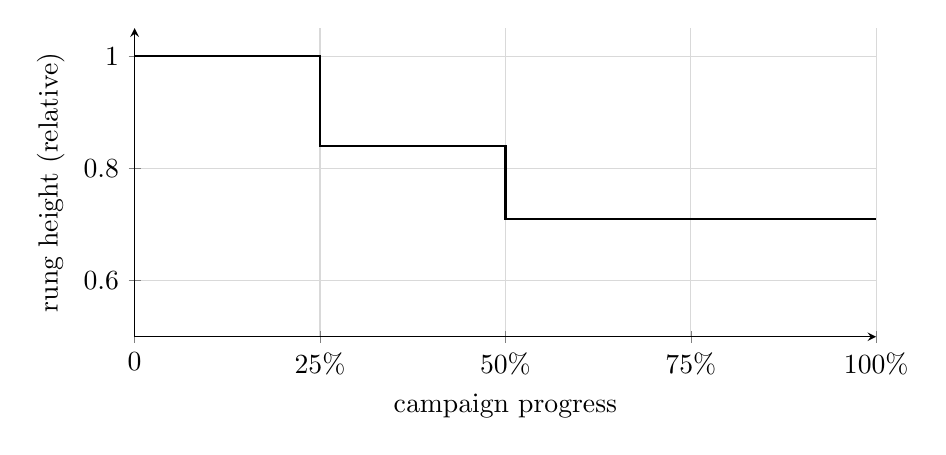
\begin{tikzpicture}
\begin{axis}[
  width=11cm, height=5.5cm,
  xlabel={campaign progress}, ylabel={rung height (relative)},
  xtick={0,0.25,0.5,0.75,1}, xticklabels={0,25\%,50\%,75\%,100\%},
  ymin=0.5, ymax=1.05,
  axis lines=left, grid=major, grid style={gray!30},
]
\addplot[color=black, thick, const plot] coordinates {(0,1.0)(0.25,0.84)(0.5,0.71)(0.75,0.71)(1,0.71)};
\end{axis}
\end{tikzpicture}
\caption{A representative recalibration path for one underperforming group: rungs step down at two
checkpoints and are frozen after the last one; a group on pace has a flat line at $1.0$.}
\label{fig:fairreach}
\end{figure}

% =====================================================================================
\section{Segments without prior history}
\label{sec:coldstart}

A segment $s$ is uninitialized if $V_s = \emptyset$. No minimum sample size is imposed: one
settled post already constitutes history for the next campaign in that segment. For an
uninitialized segment within a live campaign, the mechanism does not import rungs from a different
segment — no functional relationship between, say, gaming reels and sports reels is asserted — and
instead treats the campaign's own accruing posts as the reference population:

\begin{algorithm}
\caption{Rung construction for an uninitialized segment}
\begin{algorithmic}[1]
\State \textbf{Input:} campaign posts $\{p : s(p)=s\}$, checkpoints $\{0.25,0.5,0.75\}$
\For{$\tau \in \{0.25, 0.5, 0.75\}$}
  \State $V \gets \{v_p(\tau T) : s(p)=s,\ \text{day}(p) < \tau T\}$
  \State $\rho_s \gets$ rung construction of Def.~2 applied to $V$
  \State \textbf{if} $\tau=0.75$: freeze $\rho_s$
\EndFor
\State \textbf{Settlement:} every post in $s$, including those made before $\tau=0.25$, is paid
against the frozen $\rho_s$.
\end{algorithmic}
\end{algorithm}

Because settlement price (Eq.~\eqref{eq:settle}) requires only \emph{a} reference rate, not a
segment-specific one, and its fallback chain reaches all the way to "no reference" (plain
pool-rate settlement), coin minting in an uninitialized segment is unaffected by the absence of
rungs — every view is priced from the first campaign onward. Only the partial-credit boundary needs
a shape, and the campaign supplies its own until enough of it has been observed to freeze one; once
settled, the segment is no longer uninitialized for any later campaign.

% =====================================================================================
\section{Threshold granularity}
\label{sec:granularity}

The segment key $s = (\text{category}, \text{platform}, \text{tier}, \text{format})$ is itself a
design parameter, not a structural requirement of Sections~\ref{sec:thresholds}–\ref{sec:adaptive},
which are agnostic to what the key contains. Coarsening the key (dropping tier, say) reduces the
number of distinct ladders that must be computed, published, and defended, at the cost of pooling
accounts with structurally different reach and reintroducing exactly the cross-tier unfairness the
segmentation exists to remove. Refining the key to the individual creator is the limit case of the
same operation: it removes residual within-segment heterogeneity entirely, at the cost of the
statistical power every estimate in Sections~\ref{sec:thresholds}–\ref{sec:adaptive} depends on (a
single account's history is rarely large enough to support a stable quantile or a well-powered
binomial test) and opens a specific manipulation channel — an account can depress its own future
threshold by posting deliberately weak content early, which a shared segment ladder forecloses by
construction. The chosen operating point (category $\times$ platform $\times$ tier $\times$ format)
is the coarsest key that still respects every dimension of heterogeneity the reach model in
Section~\ref{sec:thresholds} is sensitive to; it is a point on this trade-off curve, not a value the
data selects on its own.

% =====================================================================================
\section{Empirical results}
\label{sec:results}

We evaluate the mechanism against a fixed-ladder baseline (the same absolute-view thresholds and
payouts applied uniformly to every creator, no fraud filter, no budget stop, corresponding to
current manual practice) by replaying identical realized posts under both settlement rules. Rungs,
reference rates, and fraud cut-offs for a given campaign are built only from campaigns already
settled before it began. The corpus: $120$ campaigns, $500$ creators, $4{,}251$ posts, generated by
a stochastic process with heavy-tailed per-post reach and a four-state creator behavior chain
including a purchased-views state, used identically for both settlement rules so that neither is
advantaged by the generating process.

\begin{table}[h]
\centering
\begin{tabular}{@{}lrr@{}}
\toprule
Measure & Fixed ladder & Mechanism \\
\midrule
Campaigns exceeding budget (of 120) & 22 & 0 \\
Worst overspend & $6.1\times$ budget & $0.77\times$ (never exceeded) \\
Cost per 1{,}000 genuine views (median), Rs. & 58.3 & 40.6 \\
Paid for purchased views, Rs. & $4.14\times 10^5$ & $0.90\times 10^5$ \\
Creators paid, nano tier & 19\% & 79\% \\
Creators paid, macro tier & 81\% & 74\% \\
Price dispersion across similar campaigns (CV) & 0.67 & 0.44 \\
Share of pay to top decile of creators & 50\% & 75\% \\
\bottomrule
\end{tabular}
\caption{Backtest across 120 historical campaigns, identical posts, both settlement rules.}
\label{tab:backtest}
\end{table}

Two entries in Table~\ref{tab:backtest} are directly attributable to the model's structure rather
than an incidental improvement. Macro-tier pass rates fall relative to the fixed ladder because
the segment-relative bar in Section~\ref{sec:thresholds} is, by construction, equally hard for
every tier — a flat absolute ladder is easier for large accounts precisely because it fails to
adjust for size, which is the defect being corrected. Pay concentration to the top decile rises
because settlement is proportional to credited coins rather than capped by a flat per-rung payout,
so the largest posts are paid what their reach is worth rather than clipped to a fixed rate.

Seventeen of the 120 campaigns triggered at least one recalibration event under
Section~\ref{sec:adaptive}, collectively enabling settlement for 46 creators whose posts would
otherwise have cleared no rung under the original thresholds.

% =====================================================================================
\section{Scope and limitations}
\label{sec:scope}

The budget-exactness result of Section~\ref{sec:pricing} is unconditional: it follows from
Eq.~\eqref{eq:settle} and the accounting identity in the proof of budget exactness, for any
realization of $C$, with no distributional assumption and no confidence level. The remaining
components of the mechanism are conditioned on the information available to it, and we state that
conditioning precisely rather than as a caveat.

\begin{itemize}[leftmargin=1.6em]
\item \textbf{Fraud detection is bounded by the observed signal.} The statistic in
Section~\ref{sec:fraud} is a function of daily view counts alone. Purchased views delivered slowly,
at a rate close to a creator's ordinary variance, are not separable from organic growth on this
signal; separating them requires an input the mechanism does not currently ingest (engagement or
watch-time telemetry), not a larger sample of the same input.
\item \textbf{Threshold reachability is a property of history, corrected within a campaign, not
guaranteed in advance.} Section~\ref{sec:adaptive} guarantees that a genuinely short-of-reach group
is detected and corrected \emph{during} the campaign in which it occurs; it does not guarantee the
original rung was well-calibrated at the moment it was published, only that miscalibration is
bounded and self-correcting rather than permanent.
\item \textbf{The behavioral parameter $s$ (Section~\ref{sec:thresholds}) is asserted, not
estimated.} No data on creator disengagement following a missed threshold informs its value; it is
fixed at the point equidistant between the two named failure modes absent such data, and is the
single component of this mechanism that would change in the presence of an observed
reach-to-retention relationship.
\item \textbf{The backtest holds participation fixed.} Replaying historical posts under a
counterfactual settlement rule cannot show whether a more favorable price would have changed how
many creators joined, or how many continued posting after a near miss on a threshold — that is a
property of a live market under the mechanism, not of a replay of one that ran under a different
rule.
\end{itemize}

None of the above is a precondition for the mechanism's core guarantee (budget exactness) to hold,
which is a corollary of the settlement identity, not an empirical regularity contingent on any of
the four points listed.

% =====================================================================================
\section{Conclusion}

We have specified a settlement mechanism for milestone-based creator compensation that computes a
single market-clearing price after reach is realized rather than committing to a price schedule
before it is known, derived its thin-market price as the unique Nash bargain between the realized
pool rate and an outside-option reference, placed thresholds on segment-specific empirical
quantiles of historical reach rather than on negotiated absolute numbers, given a statistical test
for withholding settlement on fabricated reach using only signals the platform itself observes, and
given a hypothesis-testing rule that corrects, within a campaign, thresholds that a specific
cohort's realized market cannot reach — while proving that its central guarantee, exact budget
adherence, follows from the settlement identity for every realization of demand, not from a
forecast of it. The mechanism requires no campaign history to begin operating in a new content
category, because coin minting and settlement pricing depend on realized reach and an outside-
option reference, neither of which requires the specific segment in question to have ever run
before.

\bibliographystyle{plainnat}
\begin{thebibliography}{9}

\bibitem[Nash(1950)]{nash1950bargaining}
J.~F. Nash.
\newblock The bargaining problem.
\newblock \emph{Econometrica}, 18(2):155--162, 1950.

\bibitem[Myerson and Satterthwaite(1983)]{myerson1983efficient}
R.~B. Myerson and M.~A. Satterthwaite.
\newblock Efficient mechanisms for bilateral trading.
\newblock \emph{Journal of Economic Theory}, 29(2):265--281, 1983.

\bibitem[Milgrom(2004)]{milgrom2004putting}
P.~Milgrom.
\newblock \emph{Putting Auction Theory to Work}.
\newblock Cambridge University Press, 2004.

\end{thebibliography}

\end{document}
